\chapter{Architektur  \label{chap_archtitektur}}
Die Netzwerkarchitektur von \ac{ITS} Stations umfasst sowohl interne als auch externe Netzwerke. Laut Standard \cite{etsi302636-3}, bzw. Standard \cite{etsi102636-3} sind dabei folgende externe Netzwerke erfasst:

\begin{itemize}
 	\item ITS ad hoc network.
	\item Access network (ITS access network, public access network, private access network).
	\item Core network (e.g. the Internet).
\end{itemize}

Auf der Grafik \ref{fig:architektur_ueberblickNetzwerke} sind die verschiedenen Netzwerke visualisiert. Diese Art der Darstellung entspricht der höchsten Abstraktionsebene. Die verschiedenen Netzwerke sind in der Grafik als Wolken dargestellt. Neben den Netzwerken sind auch die Verbindungen visualisiert.


Zusätzlich zu den hier beschriebenen Netzwerken kann eine \ac{ITS} Station ein eigenes Netzwerk, das die Teilkomponenten der \ac{ITS} Station verbindet, betreiben. Die verschiedenen Netzwerke werden benötigt, damit alle Dienste mit ihren verschiedenen Anforderungen bedient werden können.

\begin{figure}[h]
	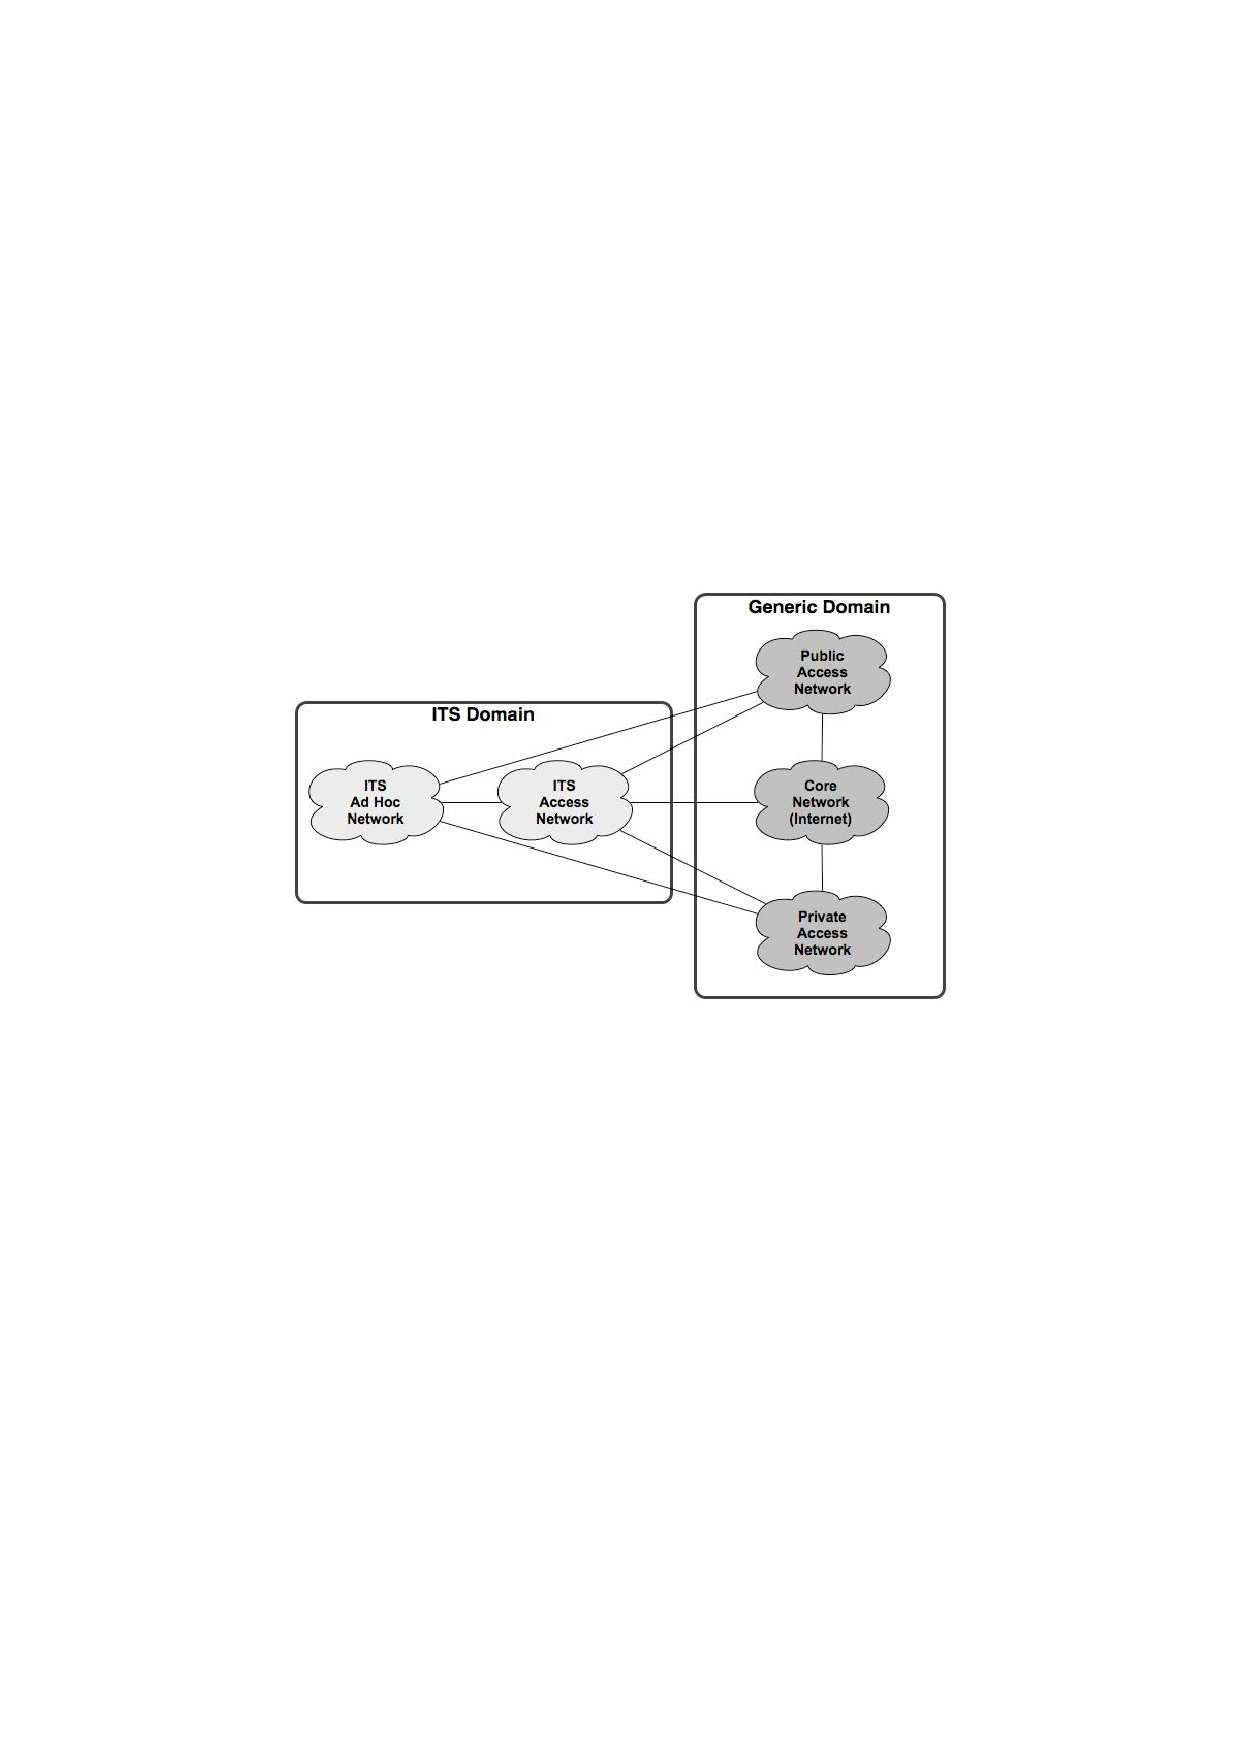
\includegraphics[width=0.99\textwidth]{content/images/02_architektur/uebersichtExterneNetzwerke.pdf}
	\caption{Überblick über die externen Netzwerke \cite{etsi302636-3}}
	\label{fig:architektur_ueberblickNetzwerke}
\end{figure}

\section{Übersicht über die verschiedenen Netzwerke}
Dieser Abschnitt soll lediglich eine Übersicht über die verwendeten Netzwerke geben. Eine weitere Erklärung der Netzwerke findet an dieser Stelle nicht statt und ist nicht Gegenstand dieser Ausarbeitung.

\subsection{ITS Ad Hoc Network}
Das \ac{ITS} Ad Hoc Netzwerk ist das Netzwerk für die Kommunikation zwischen \ac{IRS}, \ac{IVS} und \ac{PSS}. Die Kommunikation findet über die Luftschnittstelle statt. Sie ist in ihrer Reichweite begrenzt, dafür ist sie mobil einsetzbar. Die Drahtlose Kommunikation wird im Normalfall über den Standard ITS-G5 ermöglicht.


\subsection{ITS Access Network}
\tocheck{Nicht die blasseste Ahnung ob das mit den Access Networks stimmt}
ITS Access Network werden zur Vernetzung von \ac{ITS} Komponenten verwendet. Diese Netzwerke bieten 

\subsection{Public Access Network}
\subsection{Private Access Network}
\subsection{Core Network}




\section{ITS Station Reference Architecture}
Um das folgende Kapitel zu verstehen muss die \ac{ITS} Station Reference Architecture betrachtet werden. Eine Referenzarchitektur beschreibt ein allgemeines Modell einer Architektur. Das bedeutet, dass basierend auf dieser Architektur verschiedene Implementierungen existieren können. 

Die \ac{ITS} Station Reference Architecture unterscheidet sich grundlegend von bekannten Architekturen. Verglichen mit dem \ac{OSI} Modell kann man Gemeinsamkeiten erkennen:
\begin{itemize}
	\item Trennung der einzelnen Layer
	\item Definition von Service Primitiven zwischen den Layern
\end{itemize}

Bei der genaueren Beschreibung der Layer fällt auch auf, dass die Beschreibungen sich stellenweise auf das \ac{OSI} Modell beziehen. Der Hintergrund ist, dass die \ac{ITS} Station Reference Architecture an das \ac{OSI} Modell angelehnt ist. Es wurde aber um die Besonderheiten von \ac{ITS} erweitert.

Es gibt jedoch einen gravierenden Unterschied: In der \ac{ITS} Station Reference Architecture sind Cross Layer vorgesehen. Das \ac{OSI} Referenzmodell ist wasserfallartig aufgebaut. Das bedeutet, dass die einzelnen Layer übereinander angeordnet sind. Jeder Layer hat jeweils nur zu dem direkt über- und unterliegenden Layer eine Schnittstelle. Cross Layer sind Layer, die in mehrere dieser Schichten Schnittstellen haben. Im Fall der \ac{ITS} Station Reference Architecture sind das die Layer \glqq Management\grqq~ und \glqq Security\grqq. Sie haben Schnittstellen, bzw. Primitiven in alle anderen Layer. 

Möglichkeit Aufgaben dieser Layer sind:



\begin{figure}
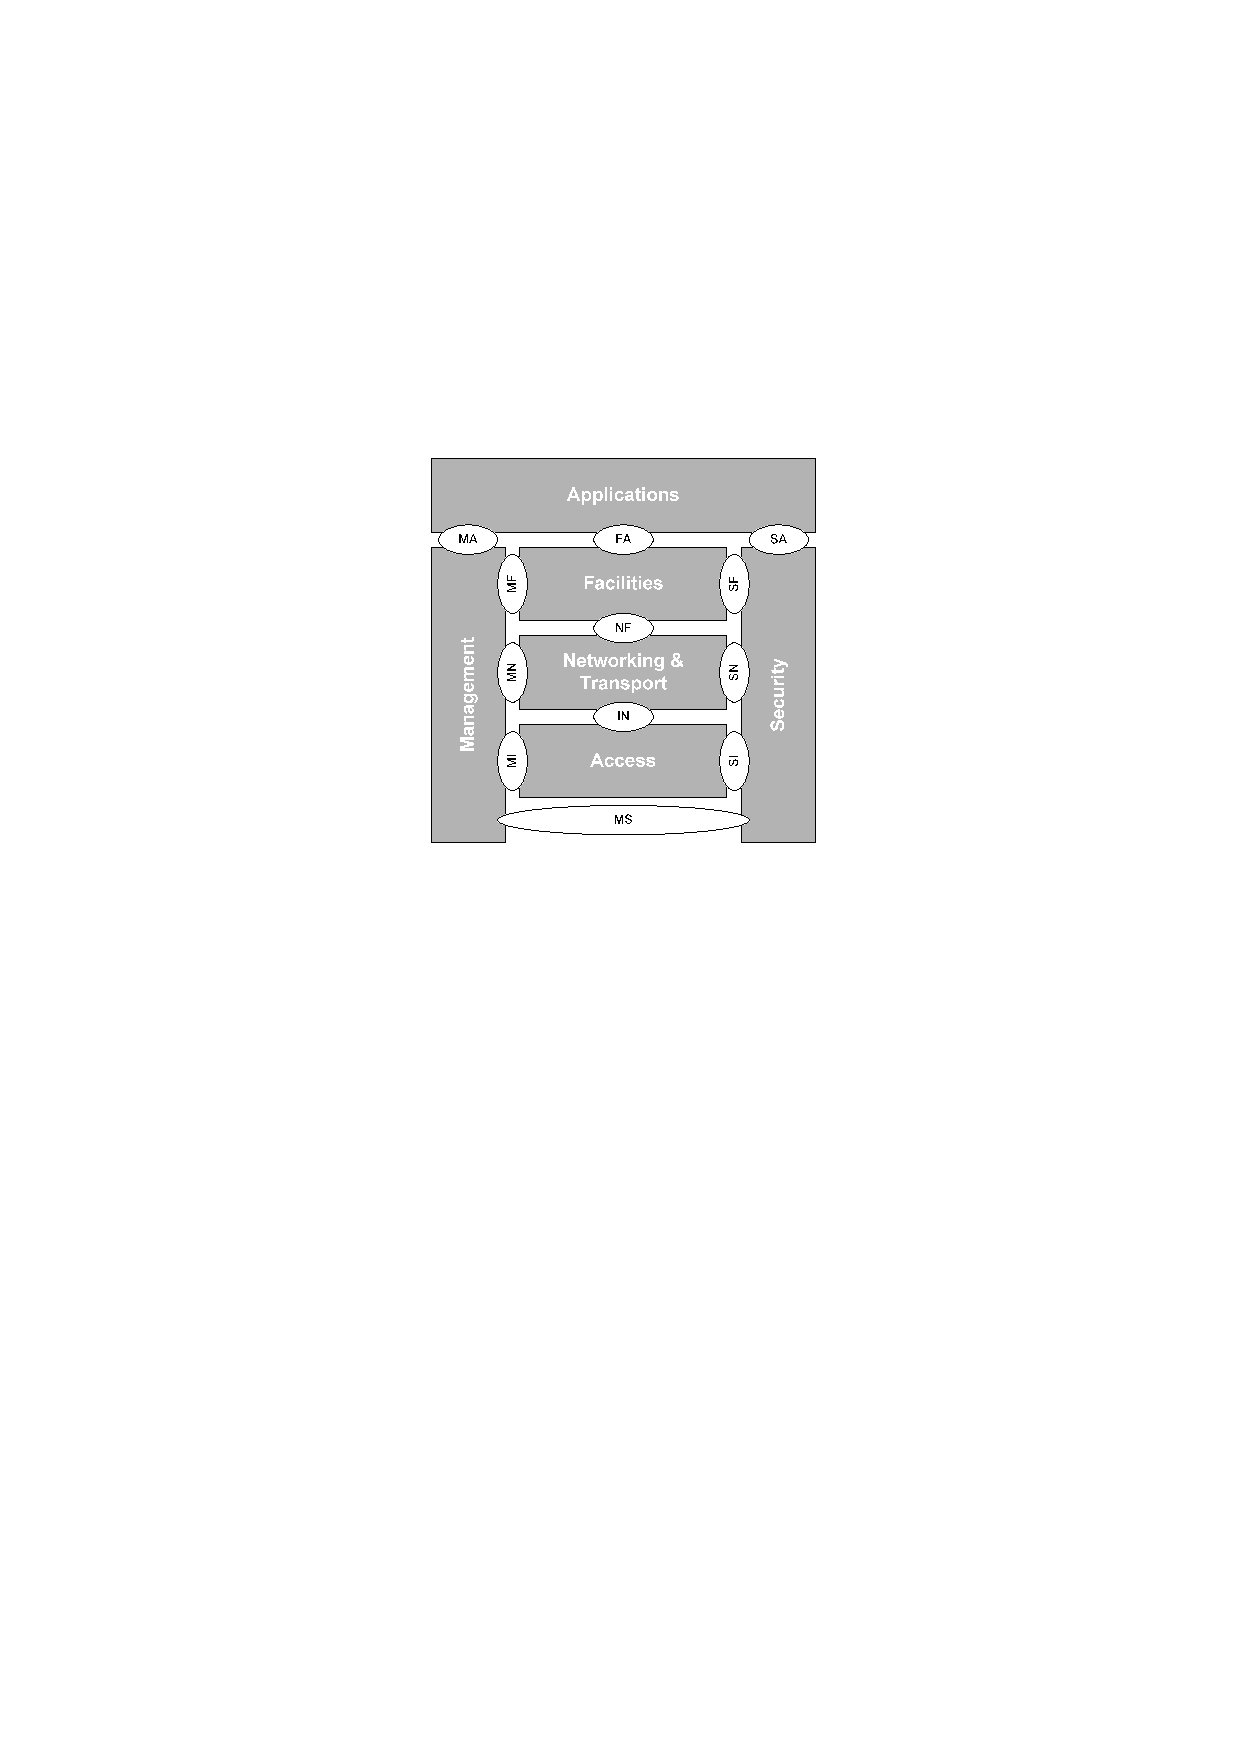
\includegraphics[width=0.75\textwidth]{content/images/02_architektur/stationReferenceArchitecture.pdf}
\caption{Darstellung der ITS Station Reference Architecture \cite{etsi2010302}}
\label{fig:funktionsweise_referenceArchitecture}
\end{figure}

\section{Wasserfall Layer}
\subsection{Access}
Der Access Layer entspricht den \ac{OSI} Layern 1 und 2. 

\subsection{Networking \& Transporting}
Der Networking \& Transporting Layer entspricht den \ac{OSI} Layern 3 und 4.

\subsection{Facilities}
Der Facilities Layer entspricht den \ac{OSI} Layern 5, 6 und 7

\subsection{Applications}


\section{Cross Layer}
\subsection{Management Layer}
Beschrieben in \cite{etsi1027232}
\todo{Management Layer genauer beschreiben}

\subsection{Security Layer}


\section{Data Security}

\section{Verwendete Protokolle}



